\documentclass[11pt]{article}
\usepackage[margin=0.75in]{geometry}
\usepackage[T1]{fontenc}
\usepackage{lmodern}
\usepackage{booktabs}
\usepackage{listings}
\usepackage{graphicx}
\usepackage{xcolor}
\usepackage{amsmath}
\usepackage[colorlinks=true,linkcolor=blue,citecolor=blue,urlcolor=blue]{hyperref}

\lstset{basicstyle=\ttfamily\small, columns=fixed, frame=single, breaklines=true, keepspaces=true}

% Every block I still have to write is a \TODOme{...}. Search this file for "TODO(me)".
\newcommand{\TODOme}[1]{\par\medskip\noindent
  \fcolorbox{red}{red!6}{\parbox{\dimexpr\linewidth-2\fboxsep-2\fboxrule\relax}{%
  \textbf{\textcolor{red}{TODO(me):}} #1}}\par\medskip}
\newcommand{\pair}[2]{#1$\to$#2}
\newcommand{\cand}[1]{\texttt{#1}}

\newcommand{\OpMatch}{208}
\newcommand{\OpPairs}{208}
\newcommand{\OpStates}{1,556}


\title{Inferring the Memory Models of the Apple M4 and the Samsung S25 Ultra from Litmus Tests}
\author{Vaishnavi Jadhav (\href{mailto:vjadh4@uic.edu}{vjadh4@uic.edu})\\
  CS 554 final report\\
  Repo: \url{https://github.com/VaishJadhavVJ/memory-model-inference}}
\date{December 2026}

\begin{document}
\maketitle

% =====================================================================================
\section{Introduction and goal}

% TODO(me)
\TODOme{Write the introduction (about half a page). Hints from the proposal, as recorded in
CLAUDE.md and notes.md (\texttt{docs/proposal.pdf} is not in the repo yet, so check them against it):
\begin{itemize}
  \item The two questions: (1) Is the M4 in Arm mode as weak as the Arm specification allows?
        (2) Does its hardware TSO mode match x86-TSO?
  \item The proposal (Oct 23) predicted that the M4 in Arm mode preserves \pair{R}{W} order,
        citing Khayet and Morrison~\cite{khayet2026}.
  \item The method: treat the chip as a black box, run litmus tests on it with litmus7, and compare
        what it does with what candidate models allow according to herd7.
\end{itemize}}

% =====================================================================================
\section{Background}

\paragraph{Litmus tests.} A litmus test is a tiny concurrent program: two to four threads with a
few loads and stores each, an initial state, and a final condition (\texttt{exists}) that names one
\emph{weak outcome}. herd7~\cite{herdtools7,herdingcats} decides whether a memory model allows that
outcome (A) or forbids it (F). litmus7~\cite{litmus2011} runs the same test millions of times on real
hardware and counts how often the outcome appears. Our tests are named after their shapes: SB (store
buffering), MP (message passing), LB (load buffering), 2+2W, S, WRC and IRIW, plus coherence tests
(CoRR, CoWR, CoRW, CoWW) that use a single location.

\paragraph{Models.} We wrote each model as a herd7 \texttt{.cat} file.
\begin{itemize}
  \item \textbf{SC} (sequential consistency~\cite{lamport1979}): all accesses happen in one global
        order that respects every thread's program order.
  \item \textbf{TSO} (as in x86-TSO~\cite{x86tso}): like SC, except that a store may be delayed past
        later loads of the same thread (a store buffer), so \pair{W}{R} order is not kept.
  \item \textbf{RLX}: only coherence. Each location on its own behaves like SC; nothing else is ordered.
  \item \textbf{RA} (release/acquire~\cite{lahav2016}): if a thread reads a value, it also sees everything
        that happened before that write (happens-before is program order plus reads-from, chained).
        Different readers may disagree on the order of independent writes.
  \item \textbf{SRA} (strong release/acquire~\cite{lahav2016}): RA, plus writes are ordered consistently
        with happens-before.
  \item \textbf{Arm}: herd7's built-in \texttt{aarch64.cat}, Arm's axiomatic model. Armv8 is multi-copy
        atomic~\cite{pulte2018}: a store becomes visible to all other threads at once. Independent
        accesses to different locations may be reordered, but dependencies, barriers and
        acquire/release instructions create order.
\end{itemize}

% =====================================================================================
\section{Method}

\subsection{The 13-test suite and its validation}
Nine tests were generated with diyone7 (herdtools7 7.58): SB, MP, LB, 2+2W, S, WRC, IRIW, and
LB+datas and IRIW+addrs, which add a data or address dependency to LB and IRIW. Four coherence tests
(CoRR, CoWR, CoRW, CoWW) were generated with \texttt{diyone7 -oneloc}. For CoWR, CoRW and CoWW,
diyone7 wrote the final condition in the wrong order, so CoRW and CoWW came out allowed even under SC.
We kept diyone7's code and rewrote only the \texttt{exists} line of those three tests, recording the
original condition in a \texttt{Fix=} header line.

To check that every weak outcome is reachable at all, we wrote \texttt{none.cat}, a model with no
axioms. All 13 tests are allowed under it, so whenever a model forbids a test, the reason is the
model's rules, not a broken test.

\subsection{Baselines and the 16 candidates}
The baselines are our own \texttt{none.cat}, \texttt{rlx.cat}, \texttt{ra.cat}, \texttt{sra.cat},
\texttt{tso.cat} and \texttt{sc.cat}, plus herd7's \texttt{aarch64.cat}. The 16 candidates have the shape
of \texttt{tso.cat}: a coherence axiom plus
$\mathit{acyclic}(\mathit{ppo} \cup \mathit{rfe} \cup \mathit{co} \cup \mathit{fr})$, where
$\mathit{ppo}$ keeps the program-order pairs whose flag is set. There is one yes/no flag per pair kind:
\pair{W}{W}, \pair{W}{R}, \pair{R}{R} and \pair{R}{W} (different locations, dependencies ignored).
A candidate is named by its flags, for example \cand{cand\_WW0\_WR0\_RR0\_RW1} (only \pair{R}{W} kept),
written 0001 for short.

\texttt{scripts/check\_predictions.py} checks the predictions automatically (15 checks, all pass):
the all-ones candidate equals \texttt{sc.cat} and \cand{cand\_WW1\_WR0\_RR1\_RW1} equals \texttt{tso.cat}
on all 13 tests; every candidate forbids the four coherence tests; no two candidates agree on every
test; SB, 2+2W, LB and IRIW are forbidden exactly when \pair{W}{R}, \pair{W}{W}, \pair{R}{W} and
\pair{R}{R} respectively are kept; LB+datas equals LB and IRIW+addrs equals IRIW for every candidate;
and the five Phase 1 results of Section~\ref{sec:phase1}.

\subsection{Inference rules}
For each candidate and each test:
\begin{itemize}
  \item \textbf{Hard evidence.} If the hardware showed the weak outcome but the candidate forbids it,
        the candidate is eliminated.
  \item \textbf{Soft evidence.} If the candidate allows the outcome but the hardware never showed it,
        the candidate survives and the test counts as a \emph{mismatch}. ``Never seen'' can also mean
        ``allowed but rare''.
\end{itemize}
Survivors are ranked by their number of mismatches (\texttt{scripts/infer.py}). When a chip is run
several times, a test counts as observed if any run saw it, and the counts are summed
(\texttt{scripts/combine\_obs.py}).

\subsection{Hardware pipeline}
litmus7 turns each test into a C program, which is compiled and run on the chip. For every test,
\texttt{scripts/hw\_obs.py} checks that the hash litmus7 reports equals the hash herd7 computes for the
same file, so the hardware ran exactly the test that herd7 analysed. It then writes the weak-outcome
count and the total number of runs. All hashes matched on both chips.
\begin{itemize}
  \item \textbf{Apple M4} (10 cores: 4 performance, 6 efficiency; macOS 26.6): litmus7 with its Mac
        settings (\texttt{-mach M1}), \texttt{-a 10}, 100{,}000 iterations per run and 100 runs, which
        gives 50M runs for 2-thread tests, 30M for 3-thread tests and 20M for 4-thread tests. macOS
        cannot pin threads to cores, so threads may land on either core type.
  \item \textbf{Samsung S25 Ultra} (SM-S938B, SoC SM8750, 8 CPUs reporting two core variants, 6 + 2;
        Android kernel 6.6): a Termux package that compiles the litmus7 sources on the phone
        (\texttt{-os android8}, \texttt{-affinity random}, \texttt{-march=armv8.2-a+rcpc}) and runs each test
        at least 10M times. Two complete runs were combined, 20M runs per test.
\end{itemize}

% =====================================================================================
\section{Phase 1: simulated ground truth}\label{sec:phase1}
Before using hardware, we checked the inference on simulated observations: a test counts as
observed exactly when a known model allows it. Table~\ref{tab:phase1} shows the result.

\begin{table}[h]
\centering\small
\begin{tabular}{llll}
\toprule
Truth & Survivors & Best candidate (unique) & Mismatches \\
\midrule
SC & 16 & \texttt{cand\_WW1\_WR1\_RR1\_RW1} & 0 \\
TSO & 8 & \texttt{cand\_WW1\_WR0\_RR1\_RW1} & 0 \\
Arm (aarch64.cat) & 1 & \texttt{cand\_WW0\_WR0\_RR0\_RW0} & 2: IRIW+addrs, LB+datas \\
RA & 2 & \texttt{cand\_WW0\_WR0\_RR0\_RW1} & 3: MP, S, WRC \\
SRA & 4 & \texttt{cand\_WW1\_WR0\_RR0\_RW1} & 2: MP, WRC \\
\bottomrule
\end{tabular}

\caption{Phase 1. Each row uses one model as the ``hardware''.}
\label{tab:phase1}
\end{table}

SC and TSO lie inside the candidate space and are recovered exactly, with 0 mismatches. Arm, RA and
SRA lie outside it, and their leftover mismatches are forced, because an observed test switches off
the flag that would forbid them. They point to what the candidates cannot express: dependencies (Arm),
and causality without one global order of writes (RA, SRA).

% =====================================================================================
\section{Hardware results: Apple M4 and Samsung S25 Ultra}\label{sec:hw}

\begin{table}[h]
\centering\small
\begin{tabular}{lcrr}
\toprule
Test & aarch64.cat & M4 (weak / runs) & S25 (weak / runs) \\
\midrule
2+2W & A & 126 / 50M & 0 / 20M \\
CoRR & F & 0 / 50M & 0 / 20M \\
CoRW & F & 0 / 50M & 0 / 20M \\
CoWR & F & 0 / 50M & 0 / 20M \\
CoWW & F & 0 / 30M & 0 / 20M \\
IRIW & A & 31,177 / 20M & 88,090 / 20M \\
IRIW+addrs & F & 0 / 20M & 0 / 20M \\
LB & A & 0 / 50M & 0 / 20M \\
LB+datas & F & 0 / 50M & 0 / 20M \\
MP & A & 456 / 50M & 6 / 20M \\
S & A & 29 / 50M & 0 / 20M \\
SB & A & 2,255 / 50M & 35 / 20M \\
WRC & A & 106 / 30M & 2,228 / 20M \\
\bottomrule
\end{tabular}

\caption{Weak outcomes seen on hardware, out of all runs, with herd7's verdict for Arm.}
\label{tab:hw}
\end{table}

Neither chip showed any outcome that \texttt{aarch64.cat} forbids. On the S25, MP was seen in only one
of the two runs (6 of 10M, then 0 of 10M); following the rules above, it counts as observed.

\begin{table}[h]
\centering\small
\begin{tabular}{lllp{0.38\linewidth}}
\toprule
Chip & Surviving candidate & Mismatches & Mismatched tests \\
\midrule
M4 & \texttt{cand\_WW0\_WR0\_RR0\_RW1} & 1 & IRIW+addrs \\
M4 & \texttt{cand\_WW0\_WR0\_RR0\_RW0} & 3 & IRIW+addrs, LB, LB+datas \\
\midrule
S25 & \texttt{cand\_WW1\_WR0\_RR0\_RW1} & 1 & IRIW+addrs \\
S25 & \texttt{cand\_WW0\_WR0\_RR0\_RW1} & 3 & 2+2W, IRIW+addrs, S \\
S25 & \texttt{cand\_WW1\_WR0\_RR0\_RW0} & 4 & IRIW+addrs, LB, LB+datas, S \\
S25 & \texttt{cand\_WW0\_WR0\_RR0\_RW0} & 5 & 2+2W, IRIW+addrs, LB, LB+datas, S \\
\bottomrule
\end{tabular}

\caption{Candidates that survive on each chip, ranked by mismatches.}
\label{tab:survivors}
\end{table}

% TODO(me)
\TODOme{Interpret Tables~\ref{tab:hw} and~\ref{tab:survivors} (half a page). Hints:
\begin{itemize}
  \item LB was never seen on either chip (M4 0 of 50M, S25 0 of 20M), which matches the proposal's
        \pair{R}{W} prediction. The best fit is 0001 on the M4 and 1001 on the S25.
  \item 2+2W and S were seen on the M4 (126 and 29 of 50M) but never on the S25 (0 of 20M), which
        is why the S25's best fit also keeps \pair{W}{W}.
  \item Rates vary a lot between runs: on the S25, WRC was 3 in one run and 2225 in the other, and MP
        6 and 0.
  \item ``Never seen'' is soft evidence. Rule of three~\cite{ruleofthree}: 0 in $N$ runs gives a 95\%
        upper bound of about $3/N$ on the per-run rate (e.g.\ LB on the M4: $3/(50\text{M})$). This
        assumes independent runs, which litmus7's runs are not quite.
  \item Answer question (1) for the M4.
  \item Update the S25 numbers after the three extra runs: rerun \texttt{scripts/combine\_obs.py},
        \texttt{scripts/infer.py} and \texttt{scripts/report\_tables.py}, then fix the text.
\end{itemize}}

% =====================================================================================
\section{Release/acquire extension and the C11 mapping}\label{sec:ra}
At Prof. Mansky's suggestion, we reran the seven shapes using Arm's release/acquire instructions.
In \texttt{+rel+acq}, every store is STLR and every load is LDAR. In \texttt{+rel+acqpc}, every store is
STLR and every load is LDAPR, the weaker acquire load (both chips support it: the M4 reports
\texttt{FEAT\_LRCPC}, the S25 lists \texttt{lrcpc}). These are the instructions that C11 release stores and
acquire loads compile to on AArch64: \texttt{memory\_order\_release} stores become STLR, and
\texttt{memory\_order\_acquire} loads become LDAR, or LDAPR on cores that have it~\cite{c11mappings}.
Our \texttt{ra.cat} treats every access as release/acquire, so it is the theoretical RA model of C11's
release/acquire fragment~\cite{lahav2016}. The 14 tests were generated with diyone7 and run with the same
settings as Section~\ref{sec:hw}; all hashes matched.

\begin{table}[h]
\centering\small
\begin{tabular}{lccccccrr}
\toprule
Test & aarch64 & RA & SRA & TSO & SC &  & M4 (weak / runs) & S25 (weak / runs) \\
\midrule
MP+rel+acq & F & F & F & F & F &  & 0 / 50M & 0 / 20M \\
SB+rel+acq & F & A & A & A & F &  & 0 / 50M & 0 / 20M \\
LB+rel+acq & F & F & F & F & F &  & 0 / 50M & 0 / 20M \\
2+2W+rel+acq & F & A & F & F & F &  & 0 / 50M & 0 / 20M \\
S+rel+acq & F & F & F & F & F &  & 0 / 50M & 0 / 20M \\
WRC+rel+acq & F & F & F & F & F &  & 0 / 30M & 0 / 20M \\
IRIW+rel+acq & F & A & A & F & F &  & 0 / 20M & 0 / 20M \\
MP+rel+acqpc & F & F & F & F & F &  & 0 / 50M & 0 / 20M \\
SB+rel+acqpc & A & A & A & A & F &  & 4,655 / 50M & 51 / 20M \\
LB+rel+acqpc & F & F & F & F & F &  & 0 / 50M & 0 / 20M \\
2+2W+rel+acqpc & F & A & F & F & F &  & 0 / 50M & 0 / 20M \\
S+rel+acqpc & F & F & F & F & F &  & 0 / 50M & 0 / 20M \\
WRC+rel+acqpc & F & F & F & F & F &  & 0 / 30M & 0 / 20M \\
IRIW+rel+acqpc & F & A & A & F & F &  & 0 / 20M & 0 / 20M \\
\bottomrule
\end{tabular}

\caption{Release/acquire tests: herd7 verdicts and weak outcomes seen on hardware.}
\label{tab:ra}
\end{table}

Facts from Table~\ref{tab:ra}: both chips match \texttt{aarch64.cat} on all 14 tests. On every test that
\texttt{ra.cat} forbids, \texttt{aarch64.cat} forbids it too. \texttt{aarch64.cat} forbids five outcomes
that RA allows: SB+rel+acq, both 2+2W variants and both IRIW variants. SB+rel+acqpc is the only
test Arm allows, and both chips showed it.

% TODO(me)
\TODOme{Interpret Table~\ref{tab:ra} (a third of a page). Hints: what ``Arm forbids everything RA
forbids'' means for compiling C11 release/acquire to STLR/LDAR/LDAPR (on these tests); why Arm is
stronger than RA (LDAR may not pass an earlier STLR; one global write order; multi-copy atomicity);
LDAPR differs from LDAR only on SB, and both chips show that difference (SB+rel+acq never, SB+rel+acqpc
seen); the two 2+2W variants are the same test, because 2+2W has no loads.}

% =====================================================================================
\section{Operational model and comparison with Arm's Flat model}\label{sec:op}
We built an operational version of the 16 candidates (\texttt{docs/opmodel.md},
\texttt{scripts/opmodel.py}). There is one shared memory, so a store is seen by every thread at once.
Each thread holds a list of its unfinished instructions. At each step, any thread may perform any
unfinished load or store, unless an earlier unfinished instruction of that thread touches the same
location, or the flag for that pair of instruction kinds is set. Exploring every order of steps gives
every reachable final state. For all 16 flag settings on all 13 tests, the set of final states equals
the full list herd7 prints for the matching candidate: \OpMatch{} of \OpPairs{} pairs, \OpStates{} states
on each side. Deliberately breaking the machine (dropping the same-location rule, or swapping the
\pair{W}{R} and \pair{R}{W} flags) makes the comparison fail, so the check is not vacuous.

% TODO(me)
\TODOme{Explain the machine in plain language (a third of a page), using the ``shared whiteboard''
picture and one or two hand simulations from \texttt{docs/opmodel.md}: SB under 0001 (both loads go
before the stores), LB under 0001 (impossible: P0's load would have to happen before itself), CoRR
(impossible for every flag setting).}

\paragraph{Comparison with Flat.} Flat~\cite{pulte2018} is Arm's operational model, implemented in
rmem~\cite{rmem}. rmem could not be installed on our Mac (its opam package needs an OCaml version
older than 4.12, which opam does not offer on Apple Silicon), so we ran Flat in the RMEM web
interface on the five tests where our machines and Arm can differ (Table~\ref{tab:flat}). Flat agrees
with \texttt{aarch64.cat} on all five. In RMEM's output, a final state marked \texttt{*>} satisfies the
test's condition; Figure~\ref{fig:rmem} shows LB+datas, where only 3 of the 4 possible final states are
reachable and none is marked.

\begin{table}[h]
\centering\small
\begin{tabular}{lcccc}
\toprule
Test & Machine 0001 (M4 fit) & Machine 1001 (S25 fit) & aarch64.cat & Flat (RMEM) \\
\midrule
LB & F & F & A & A \\
LB+datas & F & F & F & F \\
IRIW & A & A & A & A \\
IRIW+addrs & A & A & F & F \\
MP & A & A & A & A \\
\bottomrule
\end{tabular}

\caption{Our machine for the two best fits, Arm's axiomatic model, and Flat (RMEM web interface,
exhaustive search). Machine 1001 is \cand{cand\_WW1\_WR0\_RR0\_RW1}.}
\label{tab:flat}
\end{table}

\begin{figure}[h]
\centering
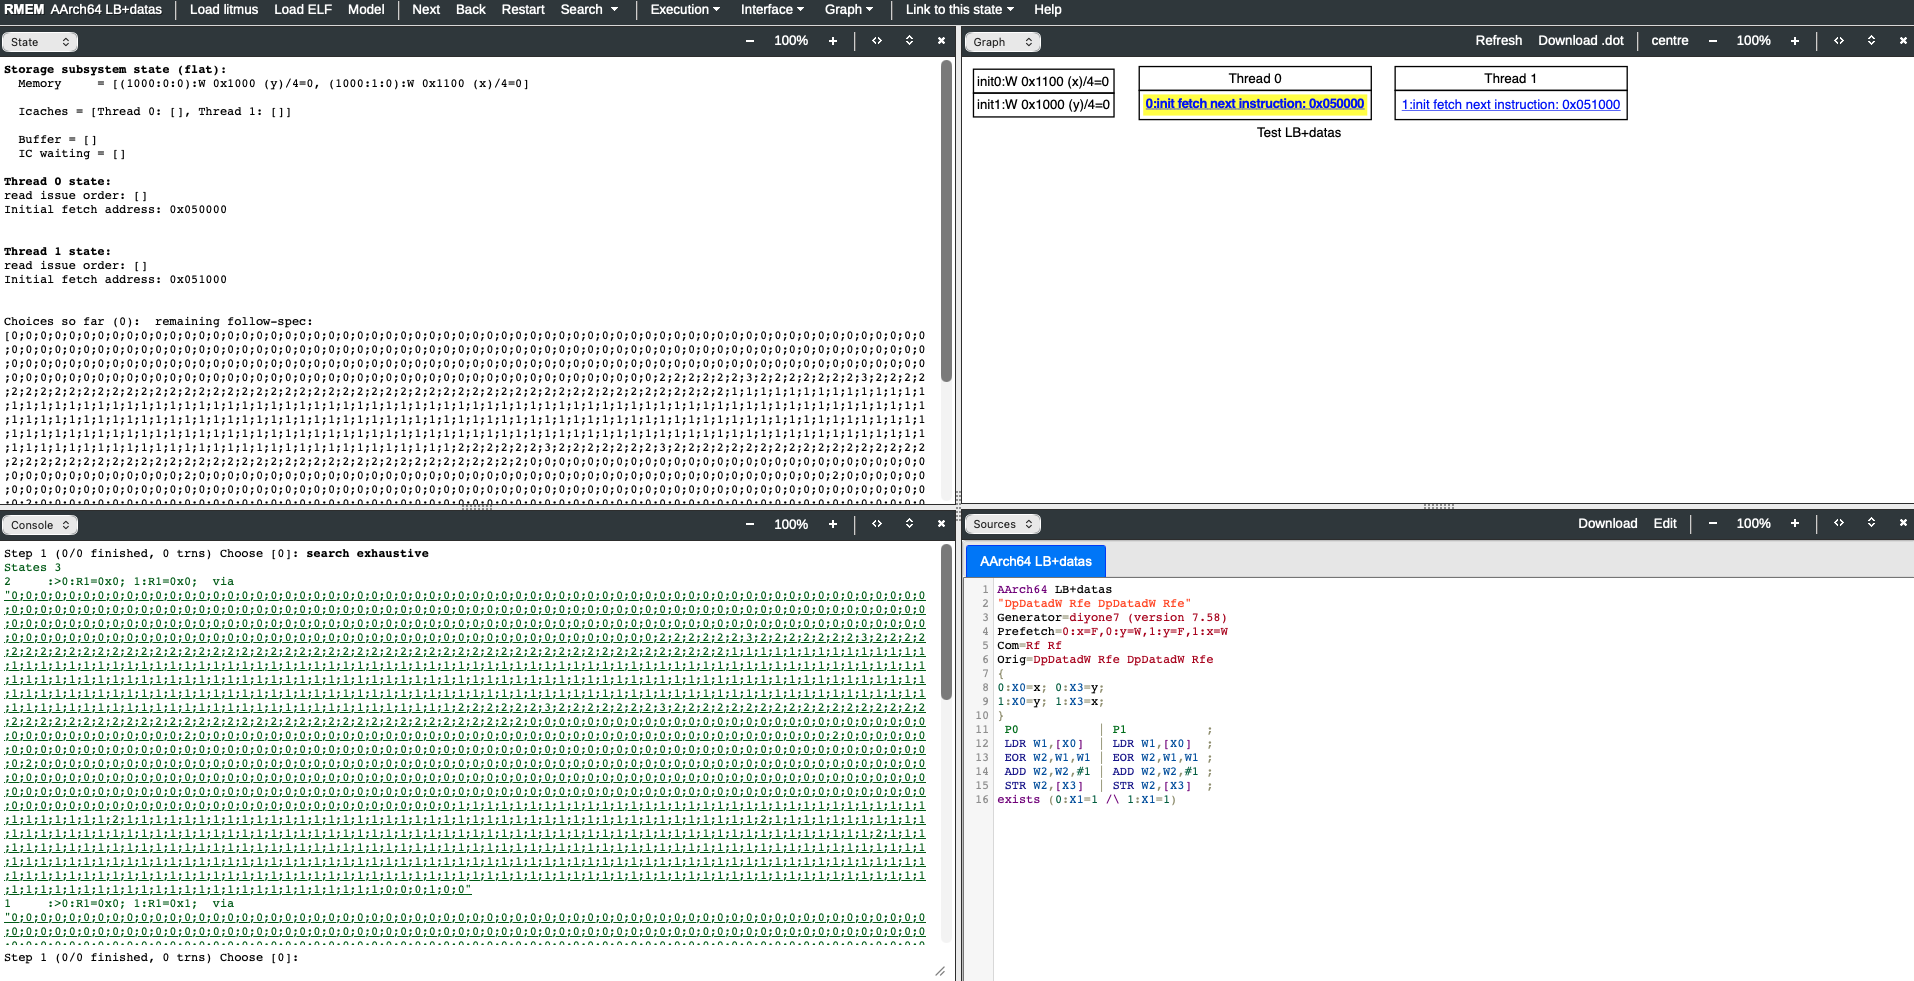
\includegraphics[width=\linewidth]{figures/flat_LB_datas.png}
\caption{RMEM web interface, Flat model, exhaustive search on LB+datas: \texttt{States 3}, and no state
satisfies the condition, so the weak outcome is forbidden.}
\label{fig:rmem}
\end{figure}

Our machines differ from Flat on LB (our \pair{R}{W} rule forbids it; Flat lets an independent store go
before an earlier load) and IRIW+addrs (Flat tracks the address dependency; our machine ignores
dependencies). Both forbid LB+datas, but for different reasons: Flat because of the data dependency,
our machines because of the \pair{R}{W} rule. Flat also models out-of-order and speculative execution,
real instruction semantics, restarts, store forwarding and barriers. Both share one flat, multi-copy
atomic memory, and both keep a thread's accesses to one location in order.

% =====================================================================================
\section{Problems and limitations}
\begin{itemize}
  \item \textbf{diyone7 conditions.} With \texttt{-oneloc}, diyone7 wrote wrong final conditions for
        CoWR, CoRW and CoWW. We fixed only the \texttt{exists} lines and validated them with
        \texttt{none.cat}.
  \item \textbf{herd7 quirks.} herd7 exits normally when a model fails to load, so our scripts stop when
        its result line is missing. It does not look for \texttt{include}d files next to the model, and it
        loads its own \texttt{sc.cat}/\texttt{tso.cat} unless given a full path.
  \item \textbf{macOS toolchain.} The Xcode license was never accepted, and the newest SDK was too new
        for the linker. We used the Command Line Tools with a matching SDK, without changing system
        settings.
  \item \textbf{No thread pinning on macOS.} M4 threads may run on performance or efficiency cores.
  \item \textbf{Android core limits.} In a first S25 attempt, Android reduced the cores available to
        Termux from 8 to 6 to 4 and refused thread pinning; CoRR then took 671 s. That run was
        incomplete and is not used.
  \item \textbf{Run-to-run variation.} Weak-outcome rates differ a lot between runs (WRC: 3 vs 2225 on
        the S25), and MP was seen in only one S25 run.
  \item \textbf{rmem.} Not installable on Apple Silicon (OCaml version constraint); Flat was run by hand on
        five tests only. RMEM's console keeps old output between tests, so the first LB+datas and
        IRIW+addrs attempts showed stale results; we reloaded the page before each test and reran them.
  \item \textbf{Limits of the candidates and the machine.} No dependencies, no barriers, and always
        multi-copy atomic, so models like Arm (dependencies) or RA (no global write order) can only be
        approximated. The machine has no store forwarding and puts all accesses in one order; neither
        matters for our 13 tests.
  \item \textbf{Soft evidence.} ``Never seen'' cannot prove ``forbidden''; the S25 has 20M runs per test
        against the M4's 20M to 50M.
\end{itemize}

% =====================================================================================
\section{What I set out to do and what I accomplished}

% TODO(me)
\TODOme{Check this table against \texttt{docs/proposal.pdf} (not in the repo yet). It is built from the
plan in CLAUDE.md, the check-in and notes.md. Fill in the reasons marked TODO.}

\begin{table}[h]
\centering\small
\begin{tabular}{p{0.34\linewidth}lp{0.44\linewidth}}
\toprule
Item & Status & Notes \\
\midrule
Phase 1: validate inference on simulated data & Done & Five truths (SC, TSO, RA, SRA, Arm); SC and TSO recovered exactly \\
Phase 2: Apple M4, Arm mode & Done & 13 tests, 20M to 50M runs each \\
Phase 3: Apple M4, TSO mode (Ubuntu VM, TSOEnabler) & Not done & TODO(me): dropped or still planned? Reason \\
Proposal prediction: M4 keeps \pair{R}{W} & Supported & LB 0 of 50M (soft evidence) \\
Stretch: Samsung S25 Ultra via Termux & Done & Two runs, 20M per test; TODO(me): three more runs \\
Pixel 8 (a friend's phone) & Not done & Package ready, no results; TODO(me): dropped or still planned? Reason \\
Stretch: LDAR/STLR tests & Done & Extended with LDAPR; 14 tests on both chips \\
Release/acquire vs theoretical RA (Prof. Mansky) & Done & Section~\ref{sec:ra} \\
Operational model (planned in OCaml) & Changed & Written in Python, like the rest of the pipeline; \OpMatch{}/\OpPairs{} match with herd7 \\
Paper proof that SB, 2+2W, LB, IRIW each pin one flag & Changed & Checked mechanically for all 16 candidates; TODO(me): add proof or drop \\
Comparison with Arm's Flat model & Changed & rmem not installable (OCaml constraint); five tests by hand in RMEM web \\
LB stress test (check-in) & Not done & TODO(me): dropped or still planned? \\
\bottomrule
\end{tabular}
\caption{Planned items and their status.}
\label{tab:plan}
\end{table}

% =====================================================================================
\section{Future work}
\begin{itemize}
  \item Stress-test LB with many more runs and other litmus7 settings, to strengthen or overturn the
        \pair{R}{W} result.
  \item Run the suite in the M4's hardware TSO mode and compare with x86-TSO (question 2).
  \item Run the Android package on more phones (e.g.\ the Pixel 8).
  \item Add dependency-aware flags to the candidates (e.g.\ \pair{R}{W} kept only when data-dependent),
        and candidates without a single global write order.
  \item Run rmem locally in a Linux VM to check all 13 tests and the release/acquire tests under Flat.
  \item Add tests with barriers (DMB).
\end{itemize}

% =====================================================================================
\section{Files in the repository and AI use}

\begin{table}[h]
\centering\small
\begin{tabular}{lp{0.62\linewidth}}
\toprule
Path & Contents \\
\midrule
\texttt{tests/}, \texttt{tests/ra/} & The 13 litmus tests and the 14 release/acquire tests \\
\texttt{models/baselines/} & \texttt{none}, \texttt{rlx}, \texttt{ra}, \texttt{sra}, \texttt{tso}, \texttt{sc} \texttt{.cat} models \\
\texttt{models/candidates/} & The 16 generated candidates \\
\texttt{scripts/} & Python (standard library only): \texttt{run\_baselines}, \texttt{gen\_candidates}, \texttt{predict},
  \texttt{predict\_ra}, \texttt{check\_predictions}, \texttt{infer}, \texttt{phase1}, \texttt{hw\_obs}, \texttt{combine\_obs},
  \texttt{opmodel}, \texttt{make\_android\_package}, \texttt{report\_tables} \\
\texttt{results/} & herd7 predictions, Phase 1 results, raw hardware logs, observation and inference CSVs,
  \texttt{opmodel\_check.csv} \\
\texttt{android/} & Termux script and instructions for running the tests on a phone \\
\texttt{docs/} & Check-in, operational model, Flat comparison, RMEM screenshots, this report \\
\texttt{notes.md} & Lab notebook: every command, result and problem, by date \\
\bottomrule
\end{tabular}
\caption{Repository layout.}
\label{tab:files}
\end{table}

\paragraph{AI use.} I used Claude for planning and Claude Code, an AI coding agent working in this
repository, for setup and implementation. Claude Code installed the tools, generated the tests with
diyone7, wrote the \texttt{.cat} models and all scripts, ran herd7 and the M4 hardware runs, built the
Android package, drafted \texttt{docs/opmodel.md}, \texttt{docs/flat\_comparison.md}, the check-in and
this report skeleton, and kept \texttt{notes.md}. I specified each step and the expected results to
check against, made the decisions when results disagreed with expectations (for example, fixing only
the coherence tests' conditions and counting MP as observed), ran the S25 tests on my phone and the Flat
tests in the RMEM web interface, and reviewed the explanations of every model and script.

% TODO(me)
\TODOme{Check that the AI-use paragraph says exactly what you did and what Claude did.}

\bibliographystyle{plain}
\bibliography{refs}

% =====================================================================================
\appendix
\section{Full prediction tables}

\begin{table}[h]
\centering\small
\begin{tabular}{lccccccccccccc}
\toprule
Model & \rotatebox{90}{2+2W} & \rotatebox{90}{CoRR} & \rotatebox{90}{CoRW} & \rotatebox{90}{CoWR} & \rotatebox{90}{CoWW} & \rotatebox{90}{IRIW} & \rotatebox{90}{IRIW+addrs} & \rotatebox{90}{LB} & \rotatebox{90}{LB+datas} & \rotatebox{90}{MP} & \rotatebox{90}{S} & \rotatebox{90}{SB} & \rotatebox{90}{WRC} \\
\midrule
\texttt{none} & A & A & A & A & A & A & A & A & A & A & A & A & A \\
\texttt{rlx} & A & F & F & F & F & A & A & A & A & A & A & A & A \\
\texttt{ra} & A & F & F & F & F & A & A & F & F & F & F & A & F \\
\texttt{sra} & F & F & F & F & F & A & A & F & F & F & F & A & F \\
\texttt{tso} & F & F & F & F & F & F & F & F & F & F & F & A & F \\
\texttt{sc} & F & F & F & F & F & F & F & F & F & F & F & F & F \\
\texttt{aarch64} & A & F & F & F & F & A & F & A & F & A & A & A & A \\
\texttt{cand\_WW0\_WR0\_RR0\_RW0} & A & F & F & F & F & A & A & A & A & A & A & A & A \\
\texttt{cand\_WW0\_WR0\_RR0\_RW1} & A & F & F & F & F & A & A & F & F & A & A & A & A \\
\texttt{cand\_WW0\_WR0\_RR1\_RW0} & A & F & F & F & F & F & F & A & A & A & A & A & A \\
\texttt{cand\_WW0\_WR0\_RR1\_RW1} & A & F & F & F & F & F & F & F & F & A & A & A & F \\
\texttt{cand\_WW0\_WR1\_RR0\_RW0} & A & F & F & F & F & A & A & A & A & A & A & F & A \\
\texttt{cand\_WW0\_WR1\_RR0\_RW1} & A & F & F & F & F & A & A & F & F & A & A & F & A \\
\texttt{cand\_WW0\_WR1\_RR1\_RW0} & A & F & F & F & F & F & F & A & A & A & A & F & A \\
\texttt{cand\_WW0\_WR1\_RR1\_RW1} & A & F & F & F & F & F & F & F & F & A & A & F & F \\
\texttt{cand\_WW1\_WR0\_RR0\_RW0} & F & F & F & F & F & A & A & A & A & A & A & A & A \\
\texttt{cand\_WW1\_WR0\_RR0\_RW1} & F & F & F & F & F & A & A & F & F & A & F & A & A \\
\texttt{cand\_WW1\_WR0\_RR1\_RW0} & F & F & F & F & F & F & F & A & A & F & A & A & A \\
\texttt{cand\_WW1\_WR0\_RR1\_RW1} & F & F & F & F & F & F & F & F & F & F & F & A & F \\
\texttt{cand\_WW1\_WR1\_RR0\_RW0} & F & F & F & F & F & A & A & A & A & A & A & F & A \\
\texttt{cand\_WW1\_WR1\_RR0\_RW1} & F & F & F & F & F & A & A & F & F & A & F & F & A \\
\texttt{cand\_WW1\_WR1\_RR1\_RW0} & F & F & F & F & F & F & F & A & A & F & A & F & A \\
\texttt{cand\_WW1\_WR1\_RR1\_RW1} & F & F & F & F & F & F & F & F & F & F & F & F & F \\
\bottomrule
\end{tabular}

\caption{herd7 verdicts for every model on the 13 tests (A = allowed, F = forbidden).}
\label{tab:predfull}
\end{table}

\begin{table}[h]
\centering\small
\begin{tabular}{lcccccccccccccc}
\toprule
Model & \rotatebox{90}{2+2W+rel+acq} & \rotatebox{90}{2+2W+rel+acqpc} & \rotatebox{90}{IRIW+rel+acq} & \rotatebox{90}{IRIW+rel+acqpc} & \rotatebox{90}{LB+rel+acq} & \rotatebox{90}{LB+rel+acqpc} & \rotatebox{90}{MP+rel+acq} & \rotatebox{90}{MP+rel+acqpc} & \rotatebox{90}{S+rel+acq} & \rotatebox{90}{S+rel+acqpc} & \rotatebox{90}{SB+rel+acq} & \rotatebox{90}{SB+rel+acqpc} & \rotatebox{90}{WRC+rel+acq} & \rotatebox{90}{WRC+rel+acqpc} \\
\midrule
\texttt{aarch64} & F & F & F & F & F & F & F & F & F & F & F & A & F & F \\
\texttt{ra} & A & A & A & A & F & F & F & F & F & F & A & A & F & F \\
\texttt{sra} & F & F & A & A & F & F & F & F & F & F & A & A & F & F \\
\texttt{tso} & F & F & F & F & F & F & F & F & F & F & A & A & F & F \\
\texttt{sc} & F & F & F & F & F & F & F & F & F & F & F & F & F & F \\
\bottomrule
\end{tabular}

\caption{herd7 verdicts on the 14 release/acquire tests.}
\label{tab:predrafull}
\end{table}

\clearpage
\section{Two example files}
\paragraph{\texttt{tests/LB.litmus}}, the test behind the main result:
\lstinputlisting{code/LB.litmus}

\paragraph{\texttt{models/candidates/cand\_WW0\_WR0\_RR0\_RW1.cat}}, the M4's best-fit candidate; all 16
candidates differ only in the \texttt{ppo} line:
\lstinputlisting{code/cand_WW0_WR0_RR0_RW1.cat}

\end{document}
